\documentclass[tikz, border=8pt]{standalone}
\usepackage{tikz}
\usetikzlibrary{arrows.meta, calc}

\begin{document}
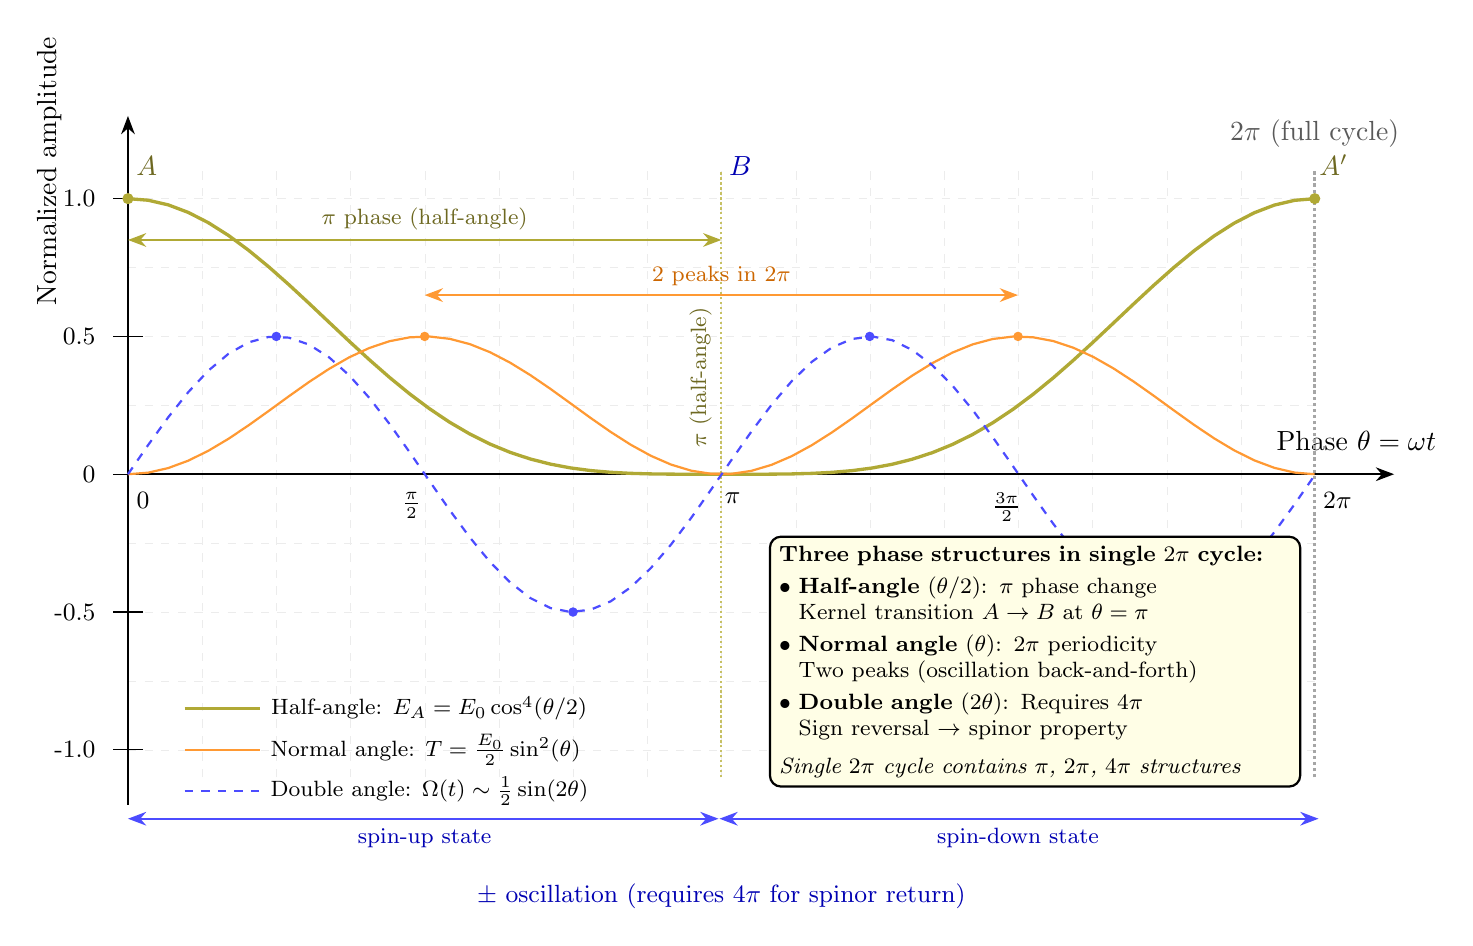
\begin{tikzpicture}[
    x=2.4cm,
    y=3.5cm,
    >=Stealth
]
    \draw[gray!15, xstep=0.3927, ystep=0.25, dashed, very thin] (0,-1.1) grid (6.28, 1.1);
    \draw[thick, ->] (0,0) -- (6.7,0);
    \draw[thick, ->] (0,-1.2) -- (0,1.3);
    \node[font=\normalsize, anchor=south] at (6.5, 0.05) {Phase $\theta = \omega t$};
    \node[font=\normalsize, anchor=south, rotate=90] at (-0.3, 1.1) {Normalized amplitude};
    \foreach \y in {-1.0, -0.5, 0, 0.5, 1.0} {
        \draw (0.08, \y) -- (-0.08, \y);
        \node[left, font=\small] at (-0.12, \y) {\y};
    }
    \node[below, font=\small, yshift=-3pt] at (0.08, 0) {$0$};
    \node[below, font=\small, yshift=-3pt] at (1.50, 0) {$\frac{\pi}{2}$};
    \node[below, font=\small, yshift=-3pt] at (3.20, 0) {$\pi$};
    \node[below, font=\small, yshift=-3pt] at (4.65, 0) {$\frac{3\pi}{2}$};
    \node[below, font=\small, yshift=-3pt] at (6.40, 0) {$2\pi$};
    \draw[olive!50, densely dotted, thick] (3.14, -1.1) -- (3.14, 1.1);
    \node[above, font=\footnotesize, olive!70!black, rotate=90, anchor=south] at (3.14, 0.35) {$\pi$ (half-angle)};
    \draw[gray!70, densely dotted, very thick] (6.28, -1.1) -- (6.28, 1.1);
    \node[above, font=\normalsize, gray!70!black] at (6.28, 1.15) {$2\pi$ (full cycle)};
    \node[above, font=\normalsize, olive!70!black] at (0.1, 1.05) {$A$};
    \node[above, font=\normalsize, blue!70!black] at (3.24, 1.05) {$B$};
    \node[above, font=\normalsize, olive!70!black] at (6.38, 1.05) {$A'$};
    \draw[olive!70, very thick, domain=0:6.28, samples=60]
        plot (\x, {(cos(\x * 180 / 3.14159 / 2)^4)});
    \filldraw[olive!70] (0, 1.0) circle (1.8pt);
    \filldraw[olive!70] (6.28, 1.0) circle (1.8pt);
    \draw[orange!80, thick, domain=0:6.28, samples=60]
        plot (\x, {0.5*(sin(\x * 180 / 3.14159)^2)});
    \filldraw[orange!80] (1.57, 0.5) circle (1.5pt);
    \filldraw[orange!80] (4.71, 0.5) circle (1.5pt);
    \draw[blue!70, thick, dashed, domain=0:6.28, samples=60]
        plot (\x, {0.5*sin(2 * \x * 180 / 3.14159)});
    \filldraw[blue!70] (0.785, 0.5) circle (1.5pt);
    \filldraw[blue!70] (3.925, 0.5) circle (1.5pt);
    \filldraw[blue!70] (2.355, -0.5) circle (1.5pt);
    \filldraw[blue!70] (5.495, -0.5) circle (1.5pt);
    \draw[<->, olive!70, thick] (0, 0.85) -- (3.14, 0.85);
    \node[above, font=\footnotesize, olive!70!black] at (1.57, 0.85) {$\pi$ phase (half-angle)};
    \draw[<->, orange!80, thick] (1.57, 0.65) -- (4.71, 0.65);
    \node[above, font=\footnotesize, orange!80!black] at (3.14, 0.65) {2 peaks in $2\pi$};
    \draw[<->, blue!70, thick] (0.000, -1.25) -- (3.125, -1.25);
    \node[below, font=\footnotesize, blue!70!black] at (1.57, -1.25) {spin-up state};
    \draw[<->, blue!70, thick] (3.130, -1.25) -- (6.3, -1.25);
    \node[below, font=\footnotesize, blue!70!black] at (4.710, -1.25) {spin-down state};
    \node[below, font=\small, blue!70!black] at (3.14, -1.45)
        {$\pm$ oscillation (requires $4\pi$ for spinor return)};
    \begin{scope}[shift={(0.3, -0.85)}]
        \draw[olive!70, very thick] (0,0) -- (0.4,0)
            node[right, font=\footnotesize, black] {Half-angle: $E_A = E_0\cos^4(\theta/2)$};
        \draw[orange!80, thick] (0,-0.15) -- (0.4,-0.15)
            node[right, font=\footnotesize, black] {Normal angle: $T = \frac{E_0}{2}\sin^2(\theta)$};
        \draw[blue!70, thick, dashed] (0,-0.3) -- (0.4,-0.3)
            node[right, font=\footnotesize, black] {Double angle: $\Omega(t) \sim \frac{1}{2}\sin(2\theta)$};
    \end{scope}
    \node[draw, thick, rounded corners, fill=yellow!10, text width=6.5cm,
          font=\footnotesize, align=left] at (4.8, -0.68) {
        \textbf{Three phase structures in single $2\pi$ cycle:}\\[2pt]
        $\bullet$ \textbf{Half-angle} $(\theta/2)$: $\pi$ phase change\\
        \phantom{$\bullet$} Kernel transition $A \to B$ at $\theta = \pi$\\[2pt]
        $\bullet$ \textbf{Normal angle} $(\theta)$: $2\pi$ periodicity\\
        \phantom{$\bullet$} Two peaks (oscillation back-and-forth)\\[2pt]
        $\bullet$ \textbf{Double angle} $(2\theta)$: Requires $4\pi$\\
        \phantom{$\bullet$} Sign reversal $\to$ spinor property\\[4pt]
        \textit{Single $2\pi$ cycle contains $\pi$, $2\pi$, $4\pi$ structures}
    };
\end{tikzpicture}
\end{document}